\documentclass[a4paper,11pt]{article}
\usepackage[left=3.0cm,right=2.5cm,top=3.0cm]{geometry}
\setlength{\parindent}{.0in}
\parskip 10pt        
\usepackage[utf8]{inputenc}
\usepackage[brazil]{babel}
\usepackage{amssymb}
\usepackage{amsthm}
\usepackage{hyperref}
\usepackage{color}
\usepackage{graphicx}
        
\newcommand{\D}{\displaystyle}
\newcommand{\mc}{\multicolumn}
\newcommand{\ft}{\footnotesize}
\newcommand{\Sc}{\scriptsize}
\newcommand{\rset}{\mathbb{R}}
\newcommand{\zset}{\mathbb{Z}}

\newcommand\SB[1]{{\color{cyan} #1}}
\newcommand\JC[1]{{\color{red} #1}}
\newcommand\AO[1]{{\color{green} #1}}

\begin{document}
\pagestyle {empty}

\vspace*{-2cm}
\begin{figure}[h]
\leavevmode
\begin{minipage}[t]{\textwidth}

\includegraphics[scale=0.7]{logo-ufrpe.eps}
\end{minipage}
\end{figure}

\vspace*{-3.0cm}
{\bf
\begin{center}
{
\hspace*{0cm} 	MINISTÉRIO DA EDUCAÇÃO E DO DESPORTO \\
\hspace*{.2in} UNIVERSIDADE FEDERAL RURAL DE PERNAMBUCO \\
\hspace*{.2in} BACHARELADO EM SISTEMAS DE INFORMAÇÃO} \\
\end{center}}
\vspace{0.0cm}
\noindent
\begin{figure}[h]
\centering
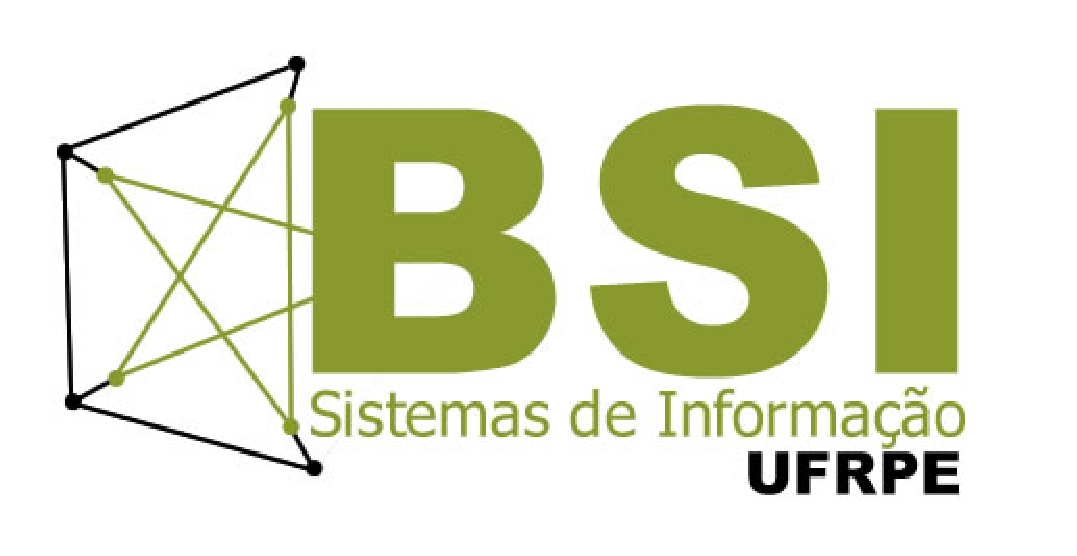
\includegraphics[scale=0.5]{Logo-bsi-presencial-v3-amp.eps}
\end{figure}
\vspace*{2.0cm}
\begin{center}

{\Large \bf  Projeto de Conclusão de Curso}\\[1cm]
{\Large \bf Título: Um Estudo sobre Desafios e Benefícios na Adoção de Métodos Ágeis por Organizações de Software} \\[3cm]
\end{center}
{\Large  Estudante: Daniel Filype Silva Barreto}\\[6mm]
{\Large  Orientador: Teresa Maciel}\\[6mm]

\vspace{3.0cm}
\begin{center}
{\large {\bf Recife}\\[6mm]
Janeiro de 2014}
\end{center}
\newpage

\newpage
\pagestyle {plain}
\setcounter{page}{0} \pagenumbering{arabic}

\section{Introdução}
\subsection{Apresentação}
O Manifesto Ágil \cite{agileManifesto}, criado em 2001, revolucionou o mercado de Tecnologia da Informação, pois, até então, a maneira de se desenvolver software mostrou-se falha em diversos aspectos. Contudo, a transição entre o modelo antigo (conhecido como "cascata") e o moderno (conhecido como "ágil") é uma tarefa não-trivial.

As principais motivações por trás da adoção ágil de desenvolvimento de software são: a melhoria da qualidade do produto final, aumento da moral dos desenvolvedores e satisfação do cliente. Entretanto, adoção ágil sempre vem com desafios especiais e, para que ela ocorra com sucesso, mudanças fundamentais na cultura da organização são necessárias \cite{Hassan2011}. Este projeto visa expor desafios e lições aprendidas por empresas brasileiras de desenvolvimento de software que passaram por este processo.
\subsection{Justificativas}
Muitas abordagens diferentes podem ser aplicadas a desenvolvimento de software \cite{Kettunen2010}, cada uma com suas peculiaridades. De acordo com \cite{Shore2007}, metodologias denominadas ágeis tornaram-se bastante populares, sendo utilizadas por grandes corporações como: Google, Yahoo!, Symantec, Microsoft, etc. Entretanto, não existe bala de prata no que tange a desenvolvimento de software. Não se deve simplesmente aplicá-las porque são populares. Existem vários estudos na literatura que mostram casos falhos de adoção de métodos ágeis \cite{Krasteva2008}. É preciso entender a fundo estas novas metodologias, analisar seus pontos positivos e negativos e, principalmente, refletir se elas agregariam valor ao produto final a ser entregue.

Sendo assim, é de suma importância a coleta de experiências para que se possa aprender sobre esta transição com aqueles que já passaram por este processo e que, além disso, querem contribuir com a comunidade de desenvolvimento de software.
\subsection{Objetivos}
\subsubsection{Objetivo Geral}
\begin{itemize}
	\item Disponibilizar um conjunto de benefícios e desafios mais relatados na adoção do desenvolvimento ágil por organizações de software.
\end{itemize}
\subsubsection{Objetivos Específicos}
\begin{itemize}
	\item Investigar, através de pesquisa exploratória, a necessidade e contribuição de trabalhos desta natureza.
	\item Adquirir conhecimento sobre fundamentos teóricos relacionados como desenvolvimento ágil de software e lean.
	\item Realizar uma revisão utilizando como base a metodologia de Revisão Sistemática \cite{Barbara2004} para coletar lições aprendidas provenientes de trabalhos publicados pela comunidade científica.
	\item Realizar uma pesquisa exploratória para coletar lições aprendidas provenientes de trabalhos publicados pela indústria de software nas principais conferências neste contexto.
	\item Identificar um conjunto de benefícios e desafios mais citados a partir dos resultados das pesquisas realizadas.
	\item Validar o trabalho realizado através de métodos de validação de Survey [ref], a partir da aplicação de questionários e entrevistas com especialistas nacionais reconhecidos na área, assim como em empresas que adotam o desenvolvimento ágil.
	\item Realizar um protótipo de um banco de dados de lições aprendidas para acesso livre pela comunidade de software.
\end{itemize}
\subsection{Organização do Trabalho}
Este trabalho é composto por mais quatro seções. Na Seção 2 está exposto uma introdução sobre metodologias ágeis. Na seção 3,  encontra-se o detalhamento da metodologia usada para realização do trabalho. O cronograma do projeto está exposto na sessão 4. Finalizando, encontram-se as referências bibliográficas de todo o material consultado para a realização deste documento.

\section{Desenvolvimento Ágil de Software}

\section{Metodologia}

\section{Cronograma}

\bibliographystyle{plain}
\bibliography{referencias}

\end{document}
